\documentclass[12pt]{article}
\usepackage{parskip}
\usepackage[nottoc]{tocbibind}
\usepackage{url}

\usepackage{graphicx}
\graphicspath{ {./img/} }

\begin{document}

    \begin{titlepage}
        \begin{center}
            \vspace{1cm}

            \LARGE
            Electronics and Computer Science\\
            Faculty of Physical Sciences and Engineering\\
            University of Southampton\\

            \Large
            \vspace{1.5cm}
            \textbf{Augustas Mirinas}\\
            December 2023

            \LARGE
            \vspace{1.5cm}
            \textbf{Trustless System for Personal Data Sharing}
            
            \vspace{1.5cm}
            \Large
            Project supervisor: George Konstantinidis\\
            g.konstantinidis@soton.ac.uk
            
            \vfill
            A project report submitted for the award of\\
            BSc Computer Science
            
        \end{center}
    \end{titlepage}

    \section*{Abstract}
    Information is appreciated in every industry. Data can be used by businesses to improve advertisement targeting, researchers process and analyze data to understand current trends and train machine learning algorithms, healthcare providers use it to offer better treatments and care. However, maintaining privacy of data subjects is a complicated issue - sharing data is an effective way to build up collective knowledge, but it also presents a threat of malicious personal data usage. In this project, current solutions to this problem are reviewed and evaluated. With the help of the consent-abiding algorithm, a new approach is proposed tackling both ability to safely share data and a way to protect sensitive information keeping it private. This progress report contains literature review, current progress and design - combination of different features from a range of systems reviewed. Actual implementation of this project is left for future work.

    \newpage
    \tableofcontents

    \newpage
    \section{Introduction}
    Companies and organizations use cloud services more than ever, meaning access to the internet user data has never been easier. Collected information is successfully used to run tailored advertising and promotions, improve customer experience or facilitate research. In this setting collected data becomes a valuable asset which can be traded and shared. This, however, comes with a serious privacy issue - after sharing their data, users lose control over it. Distributed Ledger Technology-based information sharing system can solve privacy and transparency issues by decentralizing access to collected data and giving the ability for the data owner to protect selected data attributes algorithmically.

    Data collection and sharing is also widely beneficial for healthcare and medical research. Patient information is used to prevent diseases easier, better understand their causes and risks and develop new treatments. However, medical records are sensitive information and irresponsible sharing of patient data can cause damage to the patient or his reputation. Privacy and confidentiality concerns are slowing down the progress of healthcare, and for this reason a big part of academic literature on information privacy is related to healthcare. Decentralizing systems of electronic health records (EHR) would allow to have full control for the patient over his data. Blockchain could also host the processing of stored information, respecting patient consent when sharing and querying information. This project will tackle a problem of expressing and guaranteeing user consent over personal data in trustless systems by using a distributed ledger and a fine-grained consent management algorithm described in \cite{konstantinidis}. This would guarantee shared data follows patient consent while returning the most amount of information possible. System logic hosted in a distributed ledger would make sure user constraints are being applied to every member of the system.

    \section{Literature review}
    A collection of papers on blockchain distributed ledger technologies in healthcare is reviewed and their benefits and shortcomings are considered \cite{dlt}. This, based on the mentioned research, is a review  of motivation to use blockchain for medical record management and challenges that come with it.

        \subsection{Motivation}
        The most prominent benefit of blockchain technology in any context is decentralization. Compared to a standard server-client data storage system, distributed ledger removes a threat of single point of failure. Instead of all communication relayed by a single server, which can fail and render the system useless, distributed ledger consists of multiple nodes, each having redundant data stored in them, resulting in a robust system able to handle multiple node failures and always available. Peer-to-peer approach also enables the system to be independent of any third-party data storages - meaning the information and logic of the system is not owned by anyone. The distributed ledger is managed by collaborating parties each following the blockchain protocol - "independently managed healthcare stakeholders collaborate with one another without ceding control to a central management intermediary" \cite{dlt}.

        Another benefit of storing and sharing medical records in a distributed ledger is immutability. In Bitcoin \cite{bitcoin} blockchain (used as an example in \cite{dlt}) it is achieved by each node checking every new transaction matches with the already completed ones. The decision is made by the majority of nodes - meaning once the transaction is accepted and mined, it is very difficult to change or remove it. This means blockchain ledger only supports read and write operations - ensuring data immutability and traceability. Electronic health records could use this blockchain property not only for the medical data, but for patient preferences of data sharing as well.

        Some implementations of blockchain distributed ledgers have "smart contracts", which enables to carry out computation on the blockchain. Smart contracts are set of rules stored in the blockchain, which can be triggered by a blockchain member or when other conditions are met. Instead of servers managing access to patient data, blockchain would independently return data complying with patient data sharing preferences. A smart contract would write completed queries to a blockchain to produce a log of interactions with the patient data.

        \subsection{Challenges and solutions}
        Ledger decentralization and immutability are enabled by every participating node accessing every blockchain transaction - this creates a data privacy issue. To solve this issue indexes of patient data should be stored in the blockchain, together with patient data sharing preferences. The collected data itself should be stored off-blockchain, possibly in a cloud storage for better scalability. All sensitive information stored in the blockchain should be encrypted. This implementation solves the issue of confidentiality.

        Another safety threat is a 51\% attack on a blockchain. Because new blocks are approved by the majority of nodes, a malicious actor controlling 51\% of blockchain computation power would have the ability to approve invalid blocks. The solution to this problem is a permissioned blockchain, as described in \cite{permissioned}. Approved healthcare workers, researchers and other authorized institutions would form a distributed ledger, every interaction with patient data recorded in the blockchain by a smart contract. This environment does not allow to control majority of nodes for any blockchain member and makes the 51\% attack improbable.

        Last concerns common to all blockchain-based systems are speed and scalability. Paper mentioned above uses Bitcoin blockchain for consideration, which uses Proof-of-work consensus mechanism to validate new blocks \cite{dlt}. This approach requires complicated computation to approve transactions, which limits the maximum amount of transactions per second and uses a lot of computing power. However, in recent years more effective protocols have been implemented. By choosing more optimal consensus mechanism for the blockchain in consideration, transaction completion speed might be sufficient.

        \subsection{System attributes}
        First thing to decide when considering a data sharing system is the storing of information. Most standard way to store information is cloud-based services. Cloud storage does not require initial capital to buy, setup and maintain on-premise databases, it also has practically unlimited space and the price for this service depends on the amount of information stored - meaning this solution is highly scalable. With appropriate permissions, data from the cloud can be accessed anywhere, making data sharing trivial. This, however, defeats the purpose of blockchain, as data stored in cloud relies on the cloud service provider. It can also be changed by the party administrating the storage - compromising user data security. The solution is to use a private blockchain-based cloud, as done in \cite{gateways}. This technology "provides scalable, secure, highly available and independent storage service" \cite{gateways}. To protect stored sensitive data, it is encrypted with user's blockchain signature.

        Once there is a place to store data, the system needs to manage access to the data. With user signature encryption, data reading is limited to the user itself, which is simple and secure. However, when it comes to securily sharing information, there are some issues to solve. One proposed solution is profile-based access. The owner of data (the user) has full access and the ability to grant restricted access by encrypting it with a signature. To share information with other trusted parties, user can re-encrypt it to be accessible using multiple signatures. Every interaction with the data is recorded on the blockchain, which enables the user to oversee data usage and revoke any malicious access if needed by re-encrypting again, this time using user's signature only \cite{privacy}. There is a different approach, in which Ethereum \cite{ethereum} blockchain is used to analyze and format streams of data of medical devices, then pass formatted data to medical institutions and healtcare workers to take appropriate care of the patient \cite{devices}. Blockchain users receiving information do not have any control over what information is returned - computation and raw data analyzing is carried out independently on the blockchain. To adapt this architecture for compliant data sharing, queried information should be processed to exclude any attributes not consented for sharing by the user.

        One reviewed paper presents a distributed health record management system, which implements a private blockchain cloud \cite{gateways}. Access to the stored information is given through gateways and every patient controls their own gateway. Patient can control the access to each requested record, giving patient fine-grained control over his data. Access given can be temporary - after specified time, revoking is done by re-encryping patient data, similar to \cite{privacy}. This approach can be combined with G. Konstantinidis algorithm to compute "consent-abiding query answers" \cite{konstantinidis}. Instead of accepting or rejecting requests for each patient record, as done in \cite{gateways}, patients would define constraints on different nedical attributes/records and their combinations, using the algorithm proposed in \cite{konstantinidis}. It would require to store patient consent constraints on the blockchain, where only patients themselves could update their constraints. The only way to query patient information would be to request it via blockchain, enforcing consent constraints and returning compliant data only.

    \section{Design}

    To implement a system for secure private data sharing Hyperledger Fabric will be used - an "open source enterprise-grade permissioned distributed ledger technology platform"\cite{fabric}. This technology was established under the Linux Foundation, which has a reputable history of open source projects. Another useful feature is permissioned platform, meaning every member of the network knows each other. This is great for a private data sharing setting, as all members - either data subjects, data stores or data users should be approved anyway. This environment gets rid of Proof-of-work requirement, because all approved members have the same goal - provide useful information or use it for a good cause. Any action is recorded on a ledger, deterring any malicious members to take action and face consequences.
    
    % chart inspired by https://hyperledger-fabric.readthedocs.io/en/release-2.5/network/network.html
    % add labels in paragraphs depicting each graph component

    Proposed design ensures both the following of policies set by organizations and the ability to express fine-grained consent from the data owner perspective. Below is a description of major components and their role in the system.

        \subsection{Policies}
        To setup a distributed ledger with Fabric for members to join, policies must be set first. This is a way to setup the governance of a network - define which members are able to access or update the network policy, network resources, channels or smart contracts. Policy also contains requirements for the amount of member signatures to approve a resource update. Authorities in control of these updates would be organizations collecting user data. In healtchare context, this would be hospitals and other entities collecting and processing patient data. To update the network - change a smart contract or add a channel - the majority of organizations would have to endorse the change. Users submitting their data to an organization are created an indentity by the Certificate Authority of the organization. When created, users would use it to set their consent over sensitive information by writing it into the blockchain. From there, only the identity of that user could change consent constraints.

        An orderer organization can also be a centralized authority regulating private data - possibly commissions entrusted by regulating/government bodies. This would make the network even more secure and protected fom malicious organizations finding their way into the majority of authorized organizations and taking over control of the network proposed. This possibility needs further evaluation.

        \subsection{Data Sharing}
        Organizations providing collected data would store it in the form of private data - encrypted information stored off-chain while having the hash of the data on the chain. This provides a scalable solution where only the index of data is stored in the ledger. Organizations are also responsible for approval of new transactions in the distributed ledger by hosting ordering nodes participating in the process of creation and approval of new transactions. These ordering nodes would accept or reject data requests, change of patient consent and smart contract updates. Organizations can also add a peer node for information access. Once a member of the organization has been selected to host a peer node, it can also access the smart contracts to query user data. This requirement builds up the network, as users of information have to utilize their resources, in turn building up the network and making the ledger more decentralized. In practice, these nodes would be hosted by medical researches, healtcare providers wishing to access information from other organizations, businesses using data for advertisement campaigns and any parties in need for access to the data. To become a host of a peer node, an organization has to create an identity for that host and give permission for hosting, which gives full access control for organizations collecting and distributing user data.

        \subsection{Channels}
        This structure could be adapted for any industry where data sharing and privacy is relevant by creating new channels. Each channel would have a different ledger with separare ordering nodes and different organizations offering collected data. This separates the private information ledger by the type, usage or geographic locale of information. For example, hospitals' channels might be grouped by countries or even cities - sharing data between healtchare providers is mostly done between organizations situated close to each other, because patients most often use healthcare services close to their home. In this case, storing every medical record from every country in one ledger does not make a lot of sense. Channels also improve security by hosting less data in each peer. If encryption of patient data would fail for any reason, consequences would be localized. Furthermore, if there is a use case for information from multiple channels, that would simply require the peer to host a node in each channel desired - segementing ledger into channels does not create any limits for data access.

        \subsection{Chaincode}
        Different smart contracts are required for the system to maintain user data confidentiality. This includes the ability for data owners to write consent constraints into the ledger, as well as a querying function to apply consent constraints to every piece of data queried. Both processes are adapted from a personal consent algorithm proposed in \cite{konstantinidis} - queries would be processed by a smart contract applying user consent constraints, resulting in the most amount of data returned without attributes or combination of attributes breaching set privacy constraints. Each organization would have applications for using these smart contracts - access to applications would also be provided for users to set their personal data preferences.


    \section{Progress}
    Current progress has been made by reviewing literature and similar works and designing a system based on the Hyperledger Fabric technology. Big part of this project - an algorithm to express fine-grained consent - is based on the work proposed by the supervisor of this project \cite{konstantinidis}. For this reason a virtual machine has been setup containing an application with the algorithm mentioned above. This setup will be used to analyze the inner workings of the algorithm and adapt it to the distributed ledger environment. The application also contains testing functions, evaluating the algorithm against a different privacy approach, which could also be adapted to evaluate the findings of this project.

    \section{Future work}

    \vspace{1cm}
    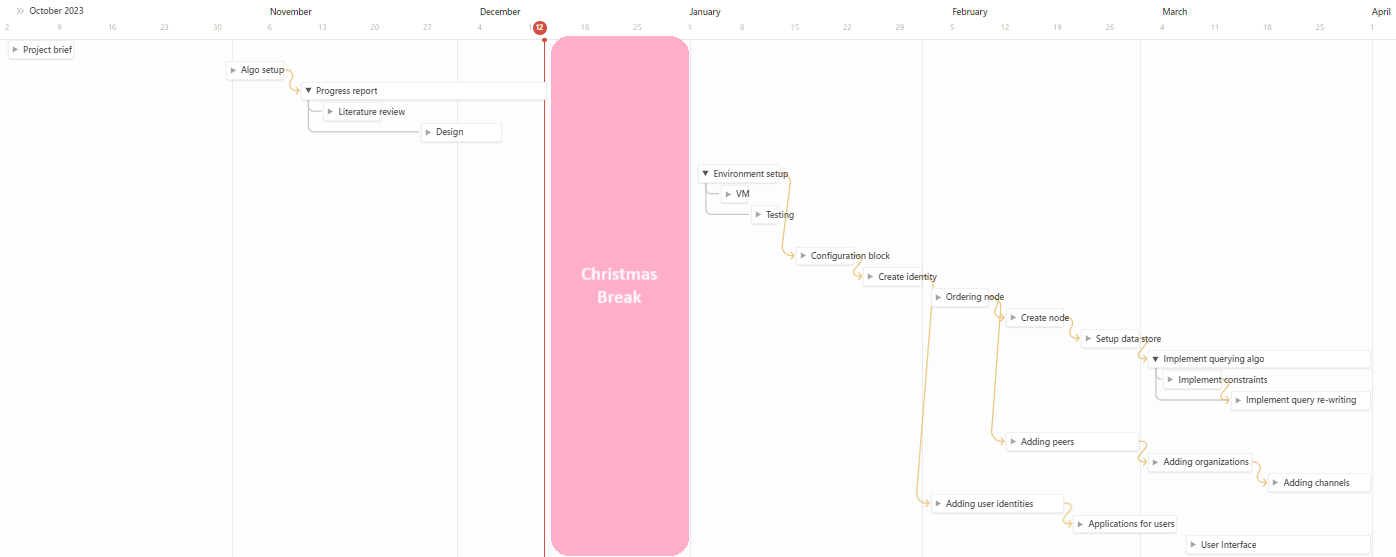
\includegraphics[width=\textwidth]{gantt.png}
    \vspace{1cm}

    Gantt chart provided includes past and future work, which might or might not be implemented in the final version of the project. The priority requirement is to have a working system with all components in place forming a distributed ledger. Once that is in place, the work will be distributed between implementing fine-grained consent algorithm and making user experience is as easy and and clear as possible. While the algorithm is at the heart of the system, a good user experience (for all parties involved) would decide how widespread and successful this system could possibly get. A gantt chart below also includes a red vertical separator dividing the past and future work at the date of this project submission.

    




    
    
    \newpage
    \bibliographystyle{ieeetr}
    \bibliography{refs}

\end{document}
